%%
%%  Department of Electrical, Electronic and Computer Engineering.
%%  EPR400/2 Project Proposal - Main File.
%%  Copyright (C) 2011-2017 University of Pretoria.
%%

\documentclass{epr400}

%% EDIT: Replace the following with your information.
\eprtitle{Design of a holonomic five legged robot}
\eprcode{EPR400}
\eprcandidatename{L. Steyn}
\eprstudentnumber{04496486}
\eprdate{November 2017}
\eprsupervisor{Dr. J.D. Le Roux}
\usepackage{placeins}
\renewcommand\cftsecaftersnum{.}
%\renewcommand\thesection{\arabic{section}}

\begin{document}

%% Include the required cover page 
\maketitlepage
%% Reset the page style and page count.
\pagestyle{fancy}
\fancyfoot{}
\renewcommand{\headrulewidth}{0pt}
\lhead{L Steyn}
\rhead{\rightmark}
\fancyfoot[R]{\thepage}
\renewcommand{\sectionmark}[1]{ \markright{#1}{} }
\pagenumbering{roman}
\setcounter{page}{1}
%Import preamble
\section*{Part 1. Preamble}
\markright{Part 1. Preamble}

This report is a description of the work I completed during the year on my final year project, Design of a holonomic five legged robot.

This report contains a copy of my approved project proposal and documentation on the technical parts of my project. These can be found in parts 3 and 4 respectively. The technical documentation contains a detailed recording of the steps taken to overcome design challenges. This includes circuit diagrams, algorithm flowcharts and test results. This section appears on the CD that accompanies this printed report.

This project does not build on any previous project. Instead it is a completely different approach to the holonomic exploration robot problem that was also addressed in earlier years. Although this project has a similar goal to that of previous years, it does not build on these as the locomotion is completely different.

This document has been language edited by a knowledgeable person. By submitting this document in its present form, I declare that this is the written material that I wish to be examined on.\\

My language editor was \_\_\_\_\_\_\_\_\_\_\_\_\_\_\_\_\_\_\_\_\\

\begin{tabular}[t]{@{}l} 
 \\ \hline \textit{Language editor signature}
\end{tabular}
\hfill% move it to the right
\begin{tabular}[t]{l@{}}
\\ \hline \textit{\hspace{15mm} Date \hspace{15mm}   } 
\end{tabular}

I,\_\_\_\_\_\_\_\_\_\_\_\_\_\_\_\_\_\_\_\_  understand  what  plagiarism  is  and  
have  carefully  studied  the  plagiarism  policy  of  the  University.  I  
hereby declare that all the work described in this report is my own, 
except  where  explicitly  indicated 
otherwise.  Although  I  may  have  
discussed the design and investigation with my study leader, fellow 
students  or  consulted  various  books,  articles  or  the  internet,  the  
design/investigative work is my own. I have mastered the design and I 
have made all the required calculations in my lab book (and/or they are  reflected  in  this  report)  to  authenticate  this.  I  am  not  
presenting a complete solution of someone else. 
Wherever  I  have  used  information  from  other  sources,  I  have  given  
credit by proper and complete referencing of the source material so 
that  it  can  be  clearly  discerned  what  is  my  own  work  and  what  was  
quoted from other sources. I acknowledge that failure to comply with 
the   instructions   regarding   referencing   will   be   regarded   as   
plagiarism.  If there is any doubt about the authenticity of my work, 
I am willing to attend an oral ancillary examination/evaluation about 
the work. 
I  certify  that  the  Project  Proposal  appearing  as  the  Introduction  
section  of  the  report  is  a  verbatim  copy  of  the  approved  Project
Proposal. \\
\begin{tabular}[t]{@{}l} 
 \\ \hline \textit{L. Steyn}
\end{tabular}
\hfill% move it to the right
\begin{tabular}[t]{l@{}}
\\ \hline \textit{\hspace{15mm} Date \hspace{15mm}   } 
\end{tabular}

%Import TOC
\newpage
\markright{Part 1. Preamble}
\tableofcontents
\thispagestyle{fancy}
%List of abbreviations
\newpage
\markright{Part 1. Preamble}
\Large{\textbf{LIST OF ABBREVIATIONS}}\\
\normalsize{}\\
\begin{tabular}{ p{5cm} l}
  \textbf{LED} & light emitting diode

\end{tabular}
%% Import the content
\section*{Part 2.}
\addcontentsline{toc}{section}{Part 2}
\markright{Part 2.}
\pagenumbering{arabic}

\cite{Hidayat:Autonomous}
%\newpage
\section*{Part 3. Project identification: approved Project Proposal}
\addcontentsline{toc}{section}{Part 3. Project identification: approved Project Proposal}
\markright{Part 3. Project Proposal}
This section contains the problem identification in the form of the complete approved Project Proposal, unchanged from the final approved version.
\newpage
%Fix the format for this section
\titleformat{\section}[frame]
{\fontsize{12pt}{14.4pt}\selectfont\bfseries} {} {5pt} {}%{\thesection\quad}
\titleformat{\subsection}[display]
{\fontsize{18pt}{21.6pt}\selectfont\bfseries} {} {5pt} {}%{\thesubsection\quad}
\titleformat{\subsubsection}[display]
{\fontsize{14pt}{16.8pt}\selectfont\bfseries} {} {5pt} {\thesubsubsection\quad}
\renewcommand\thesubsection{\arabic{subsection}.}
\renewcommand\thesubsubsection{\arabic{subsection}.\arabic{subsubsection}}
\rhead{Part 3. Project Proposal}

\begin{refsection}
%%
%%  Department of Electrical, Electronic and Computer Engineering.
%%  EPR400/2 Project Proposal - Section 1.
%%  Copyright (C) 2011-2017 University of Pretoria.
%%

\section{Problem statement}

\textbf{Motivation.}


\textbf{Context.}

\textbf{Technical challenge.}

\textbf{Limitations.}

\nocite{Haykin:Communication_Systems}

%% End of File.


%%
%%  Department of Electrical, Electronic and Computer Engineering.
%%  EPR400/2 Project Proposal - Section 2.
%%  Copyright (C) 2011-2017 University of Pretoria.
%%

\section{Project requirements}

\secunderline{ELO 3: Design part of the project}

\subsection{Mission requirements of the product}
The mission requirement of the product is
\subsection{Student tasks: design}

\vspace{1em}
\secunderline{ELO 4: Investigative part of the project}

\subsection{Research questions}

\subsection{Student tasks: experimental work}

\newpage 

%% End of File.



%%
%%  Department of Electrical, Electronic and Computer Engineering.
%%  EPR400/2 Project Proposal - Section 3.
%%  Copyright (C) 2011-2017 University of Pretoria.
%%

\section{Project plan}

This section includes the planning for the complete project period which spans over the period 1 February 2017 to 30 November 2017. The planning is in the form of a Gantt chart with a one week resolution. Figure \ref{fig:Gantt1} below shows the planning for the project up to the date of handing in this report. The blocks coloured in blue therefore represent work that is already completed.\\

\begin{figure}[htbp]
    \centering
        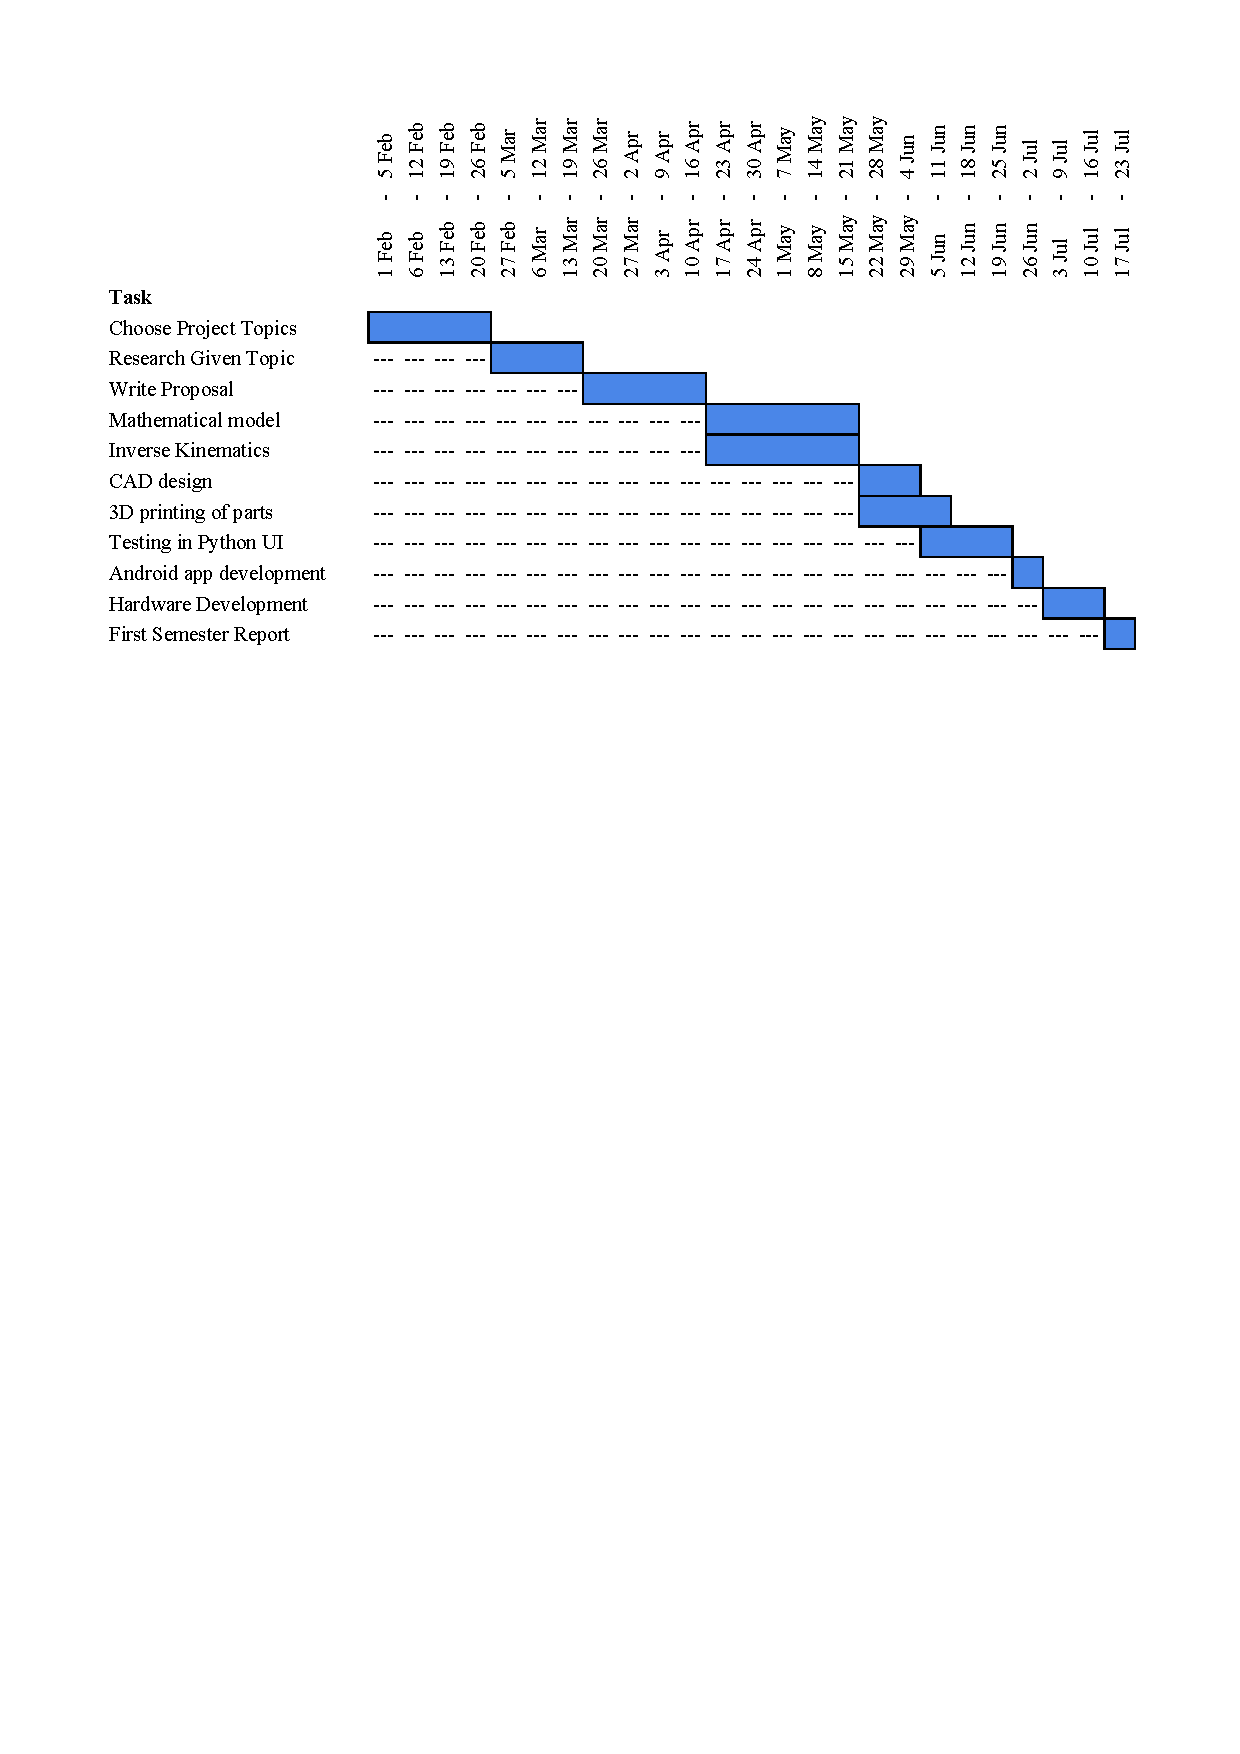
\includegraphics[clip, trim=1.5cm 18cm 1.5cm 1.5cm, width=1.00\textwidth]{pics/Gantt1.pdf}
    \caption{Gantt diagram for work already completed}
    \label{fig:Gantt1}
\end{figure}

Figure \ref{fig:Gantt2} below shows the remaining time in the project period. The blocks coloured in purple therefore represent work that still has to be completed.

\FloatBarrier
\begin{figure}[H]
    \centering
        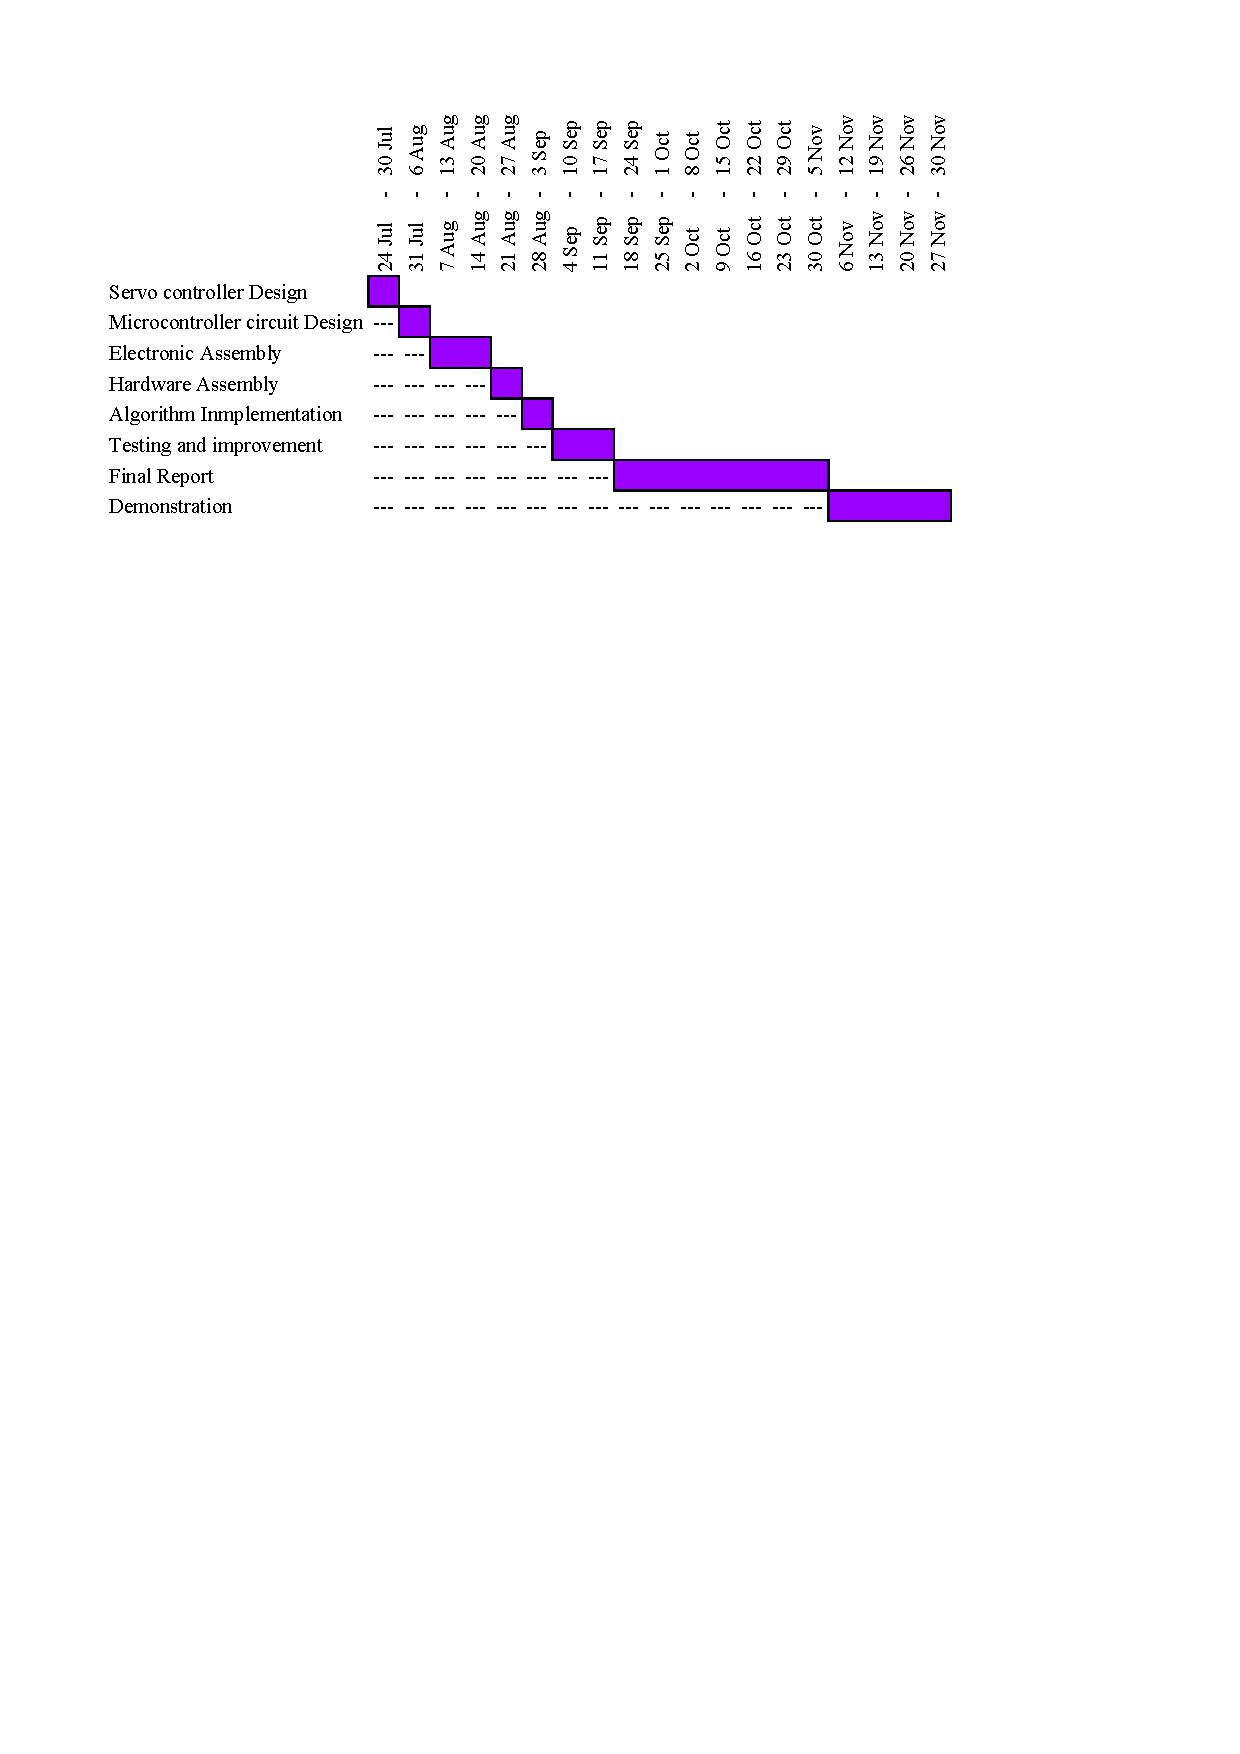
\includegraphics[clip, trim=1.5cm 21cm 1.5cm 1.5cm, width=1.00\textwidth]{pics/Gantt2.pdf}
    \caption{Gantt diagram for work to be completed}
    \label{fig:Gantt2}
\end{figure}
\FloatBarrier

%\vspace{30cm}

%\newpage

%% End of File.


%%
%%  Department of Electrical, Electronic and Computer Engineering.
%%  EPR400/2 Project Proposal - Section 4.
%%  Copyright (C) 2011-2017 University of Pretoria.
%%

\section{Specifications}

\subsection{Mission-critical system specifications}

\begin{center}
\begin{longtable}{|p{5cm}|p{5cm}|p{5cm}|}
\hline
  \textbf{SPECIFICATION (IN MEASURABLE TERMS)} &
  \textbf{ORIGIN OR MOTIVATION OF THIS SPECIFICATION} &
  \textbf{HOW WILL YOU CONFIRM THAT YOUR SYSTEM COMPLIES WITH
           THIS SPECIFICATION?}\\
\hline
   &
   &
   \\
\hline
   &
   &
   \\
\hline
   &
   &
   \\
\hline
\caption{Mission-critical system specification}
\end{longtable}
\end{center}

\subsection{Field conditions}

\begin{center}
\begin{longtable}{|p{7.5cm}|p{7.5cm}|}
\hline
  \textbf{REQUIREMENT} &
  \textbf{SPECIFICATION (IN MEASURABLE TERMS)} \\
\hline
   &
   \\
\hline
   &
   \\
\hline
   &
   \\
\hline
\caption{Field conditions}
\end{longtable}
\end{center}

\subsection{Functional unit specifications}

\begin{center}
\begin{longtable}{|p{7.5cm}|p{7.5cm}|}
\hline
  \textbf{SPECIFICATION} & \textbf{ORIGIN OR MOTIVATION} \\
\hline
   &
   \\
\hline
   &
   \\
\hline
\caption{Functional unit specifications}
\end{longtable}
\end{center}

\newpage

%% End of File.



%%
%%  Department of Electrical, Electronic and Computer Engineering.
%%  EPR400/2 Project Proposal - Section 5.
%%  Copyright (C) 2011-2017 University of Pretoria.
%%

\section*{5. Deliverables}
\addcontentsline{toc}{subsection}{5. Deliverables}

\subsection*{Technical deliverables}

\begin{center}
\begin{longtable}{|p{7cm}|p{3.5cm}|p{3.5cm}|}
\hline
\textbf{DELIVERABLE} & \textbf{DESIGNED AND IMPLEMENTED BY STUDENT} &
\textbf{OFF-THE-SHELF} \\
\hline  Microcontroller for control of the robot.
         &     & \multicolumn{1}{c|}{X}\\
\hline Control code for inverse kinematics and servo control.
         &   \multicolumn{1}{c|}{X}  &  \\
\hline Android application with a user interface for control of the robot.
         &   \multicolumn{1}{c|}{X}  &  \\
\hline Wireless module for communication between the smartphone interface and the robot
         &     &  \multicolumn{1}{c|}{X}\\
\hline Circuits implemented on PCB for interfacing all hardware with the microcontroller.
         &  \multicolumn{1}{c|}{X}   &  \\
\hline Servo motors for movement of the joints.
	&	&\multicolumn{1}{c|}{X}	\\
	\hline Robot body and legs.
	&	\multicolumn{1}{c|}{X}&	\\
	\hline Simulations on all implemented software and analogue design
	&	\multicolumn{1}{c|}{X}&	\\
\hline
\caption{Deliverables}
\end{longtable}
\end{center}

\subsection*{Demonstration at the examination}
\begin{enumerate}
\item The robot will be placed on a grid on the floor and the examiners will be shown that the robot is capable of holonomic movement.
\item The centre of the robot will be noted on the grid and the examiners will see that the robot is capable of rotating around its centre without translating.
\item The robot will execute a specific set of movements while the time to completion is being recorded.
\item Small obstacles will be placed in the way of the robot to make movement more challenging. This includes small blocks to step over as well as a change in surface such as sand.
\item The robot will repeat the set of movements over the obstacles while the time to completion is measured again.
\item The examiners will see that the robot is capable of moving with similar effort over various surfaces.
\end{enumerate}

\newpage

%% End of File.



\setcounter{subsection}{5}
\titleformat{\subsection}[frame]
{\fontsize{12pt}{14.4pt}\selectfont\bfseries} {} {5pt} {\thesubsection\quad}
\printbibliography[heading=subbibnumbered]
\end{refsection}
%Main report
\pagenumbering{arabic}
%\newpage
\setcounter{subsection}{0}
%Change formatting for tis section

\titleformat{\section}[frame]
{\fontsize{24pt}{28.8pt}\selectfont\bfseries} {} {5pt} {}
\titleformat{\subsection}[display]
{\fontsize{18pt}{21.6pt}\selectfont\bfseries} {} {5pt} {\thesubsection\quad}
\titleformat{\subsubsection}[display]
{\fontsize{14pt}{16.8pt}\selectfont\bfseries} {} {5pt} {\thesubsubsection\quad}
\renewcommand\thesubsection{\arabic{subsection}.}
\renewcommand\thesubsubsection{\arabic{subsection}.\arabic{subsubsection}}
\rhead{\rightmark}

%Start
\section*{Part 4. Main report}
\addcontentsline{toc}{section}{Part 4. Main report}
\markright{Part 4. Main report}
\secun{Literature study}
\pagenumbering{arabic}
\subsubsection{Background and context}

\subsubsection{Application of background to this project}
In this section of the report, a brief overview of the existing research that is relevant to this project will be given, as well as a short discussion on how this existing research will be used to aid in the design of a five legged holonomic robot during the course of this project.\\

Legged vehicles are preferred to wheeled vehicles for exploration and rescue in remote areas because of their ability to cross rough terrain quickly with a severely reduced risk of getting stuck. The price to pay for this superior drive-train is far more complex electronics and movement algorithms \cite{Hidayat:Autonomous}. Instead of just driving the wheel motors and steering, each limb actuator of each leg has to be controlled to move to a calculated position.\\ 

Inverse kinematics is the mathematical process used to calculate the required angles of the limbs of a structure to reach a specific set of coordinates. This is used extensively in this project because of its ability to easily transform desired Cartesian coordinates into the required actuator angles. In the paper \cite{Oh:Analytic}, a method is discussed for solving the inverse kinematic equations involved in a seven degrees of freedom robotic arm. This method takes into account specified minimum and maximum values for each actuator and degree of freedom in order to avoid self-collision. This method can be applied to any system with a specified degrees of freedom and can therefore be simplified to solve the inverse kinematic equations for the system designed in this project.\\

To obtain the Cartesian coordinates desired at any given time, the method described in \cite{Hidayat:Autonomous}, namely Sine pattern methods is used. In \cite{Hidayat:Autonomous}, the method was applied to a quadruped robot. In the case of this project, the method is expanded to make it suitable for use on a robot with five legs. Adaptation is required because the method relies on the symmetry of a quadruped robot to schedule the lifting of the legs. Since the same symmetry does not exist in a robot with five legs, a different scheduling technique is investigated. This method will rely on information from the current position of the legs, the limits of leg movement, as well as the current horizontal tilt of the robot.\\

In the conference paper \cite{Jain:Odometry}, motion planning of omnidirectional robots is discussed and a sophisticated yet simple and efficient method of route planning is proposed. This method is based on vehicles that use three omnidirectional wheels in combination to form a resultant force vector in the desired direction. These type of vehicles differ largely in terms of locomotion when compared to the holonomic legged design used in this project, but there are a few key similarities. Both these designs can move holonomically, therefore they have the ability to move in a straight line while rotating, move in an arc without rotating, or any combination of the two. These similarities mean that some of the methods discussed and applied in \cite{Jain:Odometry} can be used to aid in the design of the algorithm used in this project.\\

A team from Instituto Tecnologico de la Laguna in Mexico designed a hexapod robot \cite{Ollervides:Navigation} similar to the robot designed in this project. The purpose of the hexapod was to investigate its potential for use in exploration of areas that are hard to reach by any commonly used means of transportation. Legged vehicles are more suited to cross rough terrain, but rough terrain complicates the design of the drive-train. In applications where the surface is smooth or close to smooth, open loop control can be applied where the leg is simply moved to the desired position and it is assumed by the designer that the robot foot is making contact with the ground at this point, and therefore supporting part of the distributed robot weight. When the robot is crossing rough terrain, where the surface consists of mainly bumps and holes, this assumption could be false. In such a scenario, the robot could lift another leg while under the impression that its weight is being supported by the other legs. If this is not the case, the robot could fall over and possibly damage itself or be unable to rectify itself. To avoid this problem, closed loop control should be used in the height positioning of the legs. This involves having a sensor in the system that could provide feedback on the state of the foot. The hexapod in \cite{Ollervides:Navigation} used miniature resistive force sensors attached to the bottom of each foot of the robot. The robot therefore has the ability to take analogue measurements from these sensors and determine the weight distribution of the individual feet of the robot. This data is used to confirm that all robot feet are making contact with the surface and correct the situation if this is not the case. This type of feedback is also useful when the robot is operated on slanted surfaces because of the effect that the center of gravity has on a slanted surface. A feedback sensor will be included in the design of the five legged holonomic robot in this project.\\

If the robot is operating on a slanted surface without it being aware of this and the centre of gravity shifts over the lowest foot making contact, the robot could fall over even when all of its legs are making contact with the surface. In a paper on reactive robot navigation \cite{Arkin:Reactive}, it is proposed that the use of a digital inclinometer can aid in solving this problem. The sensor provides information on the current tilt of the robot in two dimensions. This sensor in combination with the feedback sensors on the robot feet can be used to ensure that the robot levels itself automatically to avoid tipping over. The data collected from this sensor can also be used to collect information on the terrain. In the journal article \cite{Arkin:Reactive}, this data is used for hill climbing as well as finding valleys in unexplored areas. In order to enable the robot designed in this project to walk on slanted surfaces, a digital inclinometer will be used. Some of the reactive navigation techniques discussed in \cite{Arkin:Reactive} will also be implemented to aid the robot in navigating on slanted planes.\\

In a paper on the effects of slippery surfaces on biped robots \cite{Hyeon:Reflex}, methods on avoiding falling over of a biped robot is investigated. Since these robots have to balance themselves to stay upright, an unforeseen slippery patch on a surface could be fatal for the robot. If it were possible to foresee a slippery surface, slowing down the walking gait and increasing foot surface would help increase the traction of the robot, and therefore lower the risk of slipping. Since a five legged robot is inherently stable and there is no balancing required, slippery surfaces may influence the traction of the robot but there is very low risk of falling over on level surfaces that are slippery. It is therefore suitable to just slow down movements on slippery surfaces to increase the traction where possible.

\secun{Approach}
This section outlines the initial approach to solve the functions shown in the functional block diagram. The functional block diagram of the project can be found in Figure \ref{fig:Func}
\subsubsection{Design alternatives}

\subsubsection{Preferred solution}



\secun{Design and implementation}
\subsubsection{Background}
A large part of the design of a legged robot depends on the design of a simple leg - more specifically the degrees of freedom that a single leg has. The degrees of freedom that a single leg has is determined by the amount of dimensions that the leg can make a controlled movement in, independently from any other dimensions. There are two common underlying designs in robot leg design - these are for two and three degrees of freedom respectively.\\

Figure \ref{fig:2DOF} shows an example of a common design that has two degrees of freedom. The design therefore contains two joints in one leg. In this example, the first joint is positioned vertically to form the hip op the robot leg. This allows for the side-to-side motion required for walking. The second joint is positioned horizontally to allow the lowest limb to move up and down. The two degrees of freedom controlled by this leg design is therefore the horizontal angle of the leg and the height of the foot. These two (and only these two) parameters can therefore be controlled completely independently.
\FloatBarrier
\begin{figure}[h]
\centering
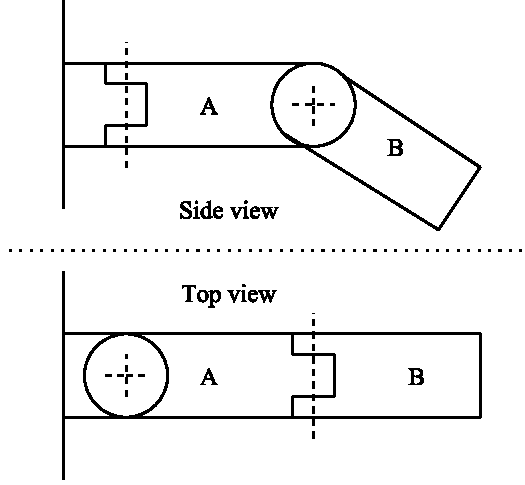
\includegraphics[scale = 1]{pics/2DOF.pdf}
\caption{Example of a leg design with two degrees of freedom.}
\label{fig:2DOF}
\end{figure}
\FloatBarrier
An example of a robotic leg with three degrees of freedom can be seen in Figure \ref{fig:3DOF}. This design is similar to that of the leg with two degrees of freedom seen in Figure \ref{fig:2DOF}, with the only addition being a second horizontal joint further down from the first. This additional limb means that the horizontal distance from the foot to the hip can be controlled as well as the height of the foot. These two controlled parameters, together with the horizontal leg angle which can also be controlled independently as in the case of the two degrees of freedom design, means that this design has a total of three degrees of freedom.
\FloatBarrier
\begin{figure}[h]
\centering
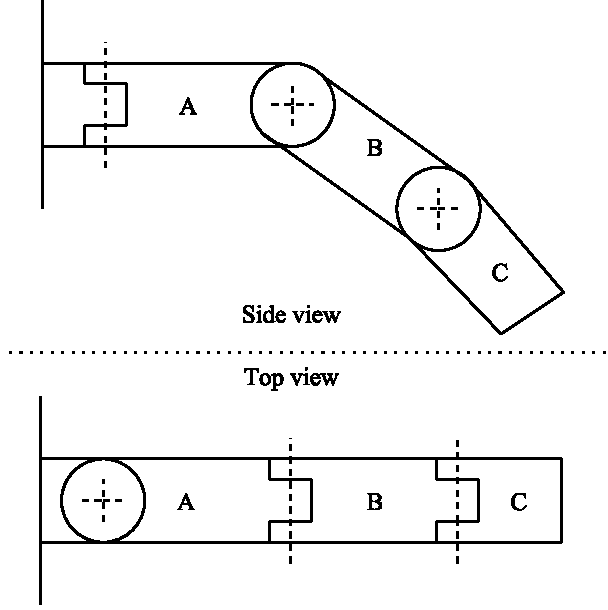
\includegraphics[scale = 1]{pics/3DOF.pdf}
\caption{Example of a leg design with three degrees of freedom.}
\label{fig:3DOF}
\end{figure}
\FloatBarrier


The design with three degrees of freedom has the advantage of being able to lift a leg without altering the horizontal position of the leg. This means that the robot is able to walk without altering the height of the body of the robot. The robot is therefore able to cross rougher terrain much better because of the ability to alter the height of the robot feet as the terrain requires. With the design that has two degrees of freedom, the foot height is a function of the horizontal extension of the leg. With this design the main advantage is the simplicity - both mechanically and in software. The cost and power consumption will also be much lower because of the reduced amount of actuators.\\

Due to the much greater flexibility of the design with three degrees of freedom and the ability to cross rougher terrain, this will be the platform implemented in the final design.\\

\subsubsection{Theoretical analysis and modelling}
\FloatBarrier
\begin{figure}[h]
\centering
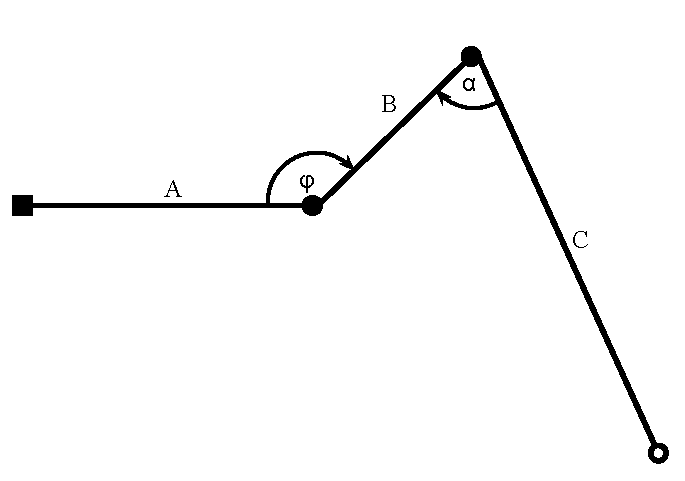
\includegraphics[scale = 1]{pics/Leg_design.pdf}
\caption{Simulation results for the network.}
\label{fig:Leg_design}
\end{figure}
\FloatBarrier

\FloatBarrier
\begin{figure}[h]
\centering
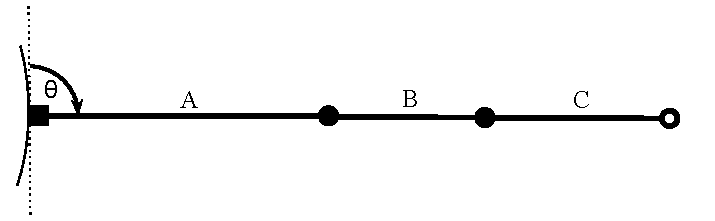
\includegraphics[scale = 1]{pics/Leg_design_2.pdf}
\caption{Simulation results for the network.}
\label{fig:Leg_design}
\end{figure}
\FloatBarrier

\subsubsection{Simulation}
\label{sec:sim}
In order to test the equations and design outlined in the Theory section above, the mathematics was implemented in a script written in the Python programming language and developed in the PyCharm IDE. The program consists of a GUI  used to enter elementary commands, similar to that implemented in the Android application, as well as a window for plotting the result in a 3-dimensional Cartesian system. Some results showing the validity of the design equations in the previous section can be found below. All of the source code used to build this simulation can be found in Part 5 of this report on the attached optical disc.\\

The program flow of the software in the simulation is similar to that used for the final prototype software, more information on the software design flow can be found in Section \ref{sec:soft}. The main difference between the final implementation and the simulation is that once the angle values for theta, alpha and phi are calculated for each leg, in the final implementation the result is used to move the actuator while in simulation the result is used to calculate the Cartesian position of each limb in order to plot it in the 3-dimensional system. It should be noted that the length of all of the limbs as well as the robot body radius was chosen as unity for simplicity and since the purpose of the simulation is only to show the functionality of the IK. It should also be noted that although some of the legs may look crooked in the following figures, this is only a result of the viewing angle. When viewed directly from above, all limbs of a single leg align in an upright plane.\\

The basic user interface together with the Robot in its neutral position can be seen in Figure \ref{fig:Sim1}.\\

The orange markers found at each of the robot feet indicate the neutral position for each of the five feet. This is indicated to aid in showing the movement of the legs relative to this neutral position in Figure \ref{fig:Sim1} and the figures following in this section.\\

\begin{figure}[H]
\centering
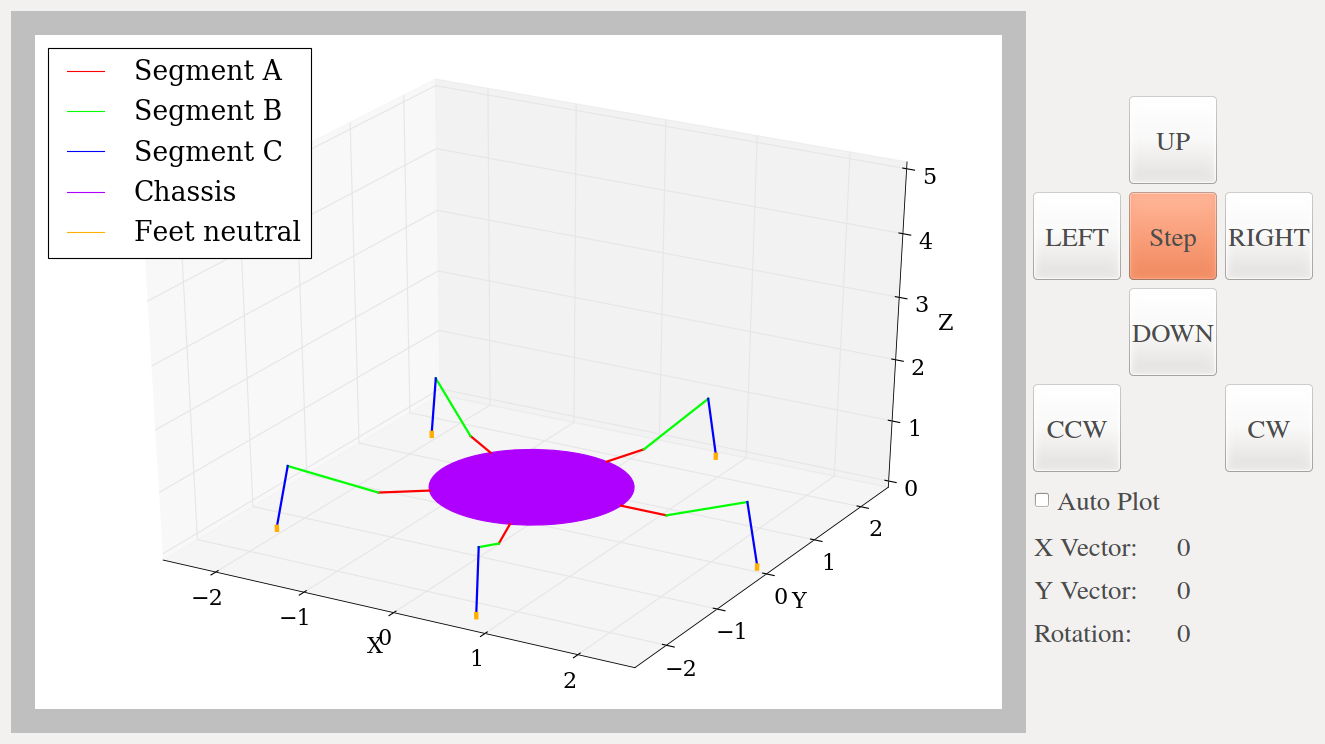
\includegraphics[scale = 0.33]{pics/Sim1.png}
\caption{Simulation window showing the robot in its neutral position.}
\label{fig:Sim1}
\end{figure}

When the $Y$ vector is changed to a positive value, the legs will all move in a negative $Y$-direction since the robot center is the origin. When the robot should move in a specific direction, the feet will move in the exact opposite direction to propel the robot forward. This is illustrated in Figure \ref{fig:Sim2}.

\begin{figure}[H]
\centering
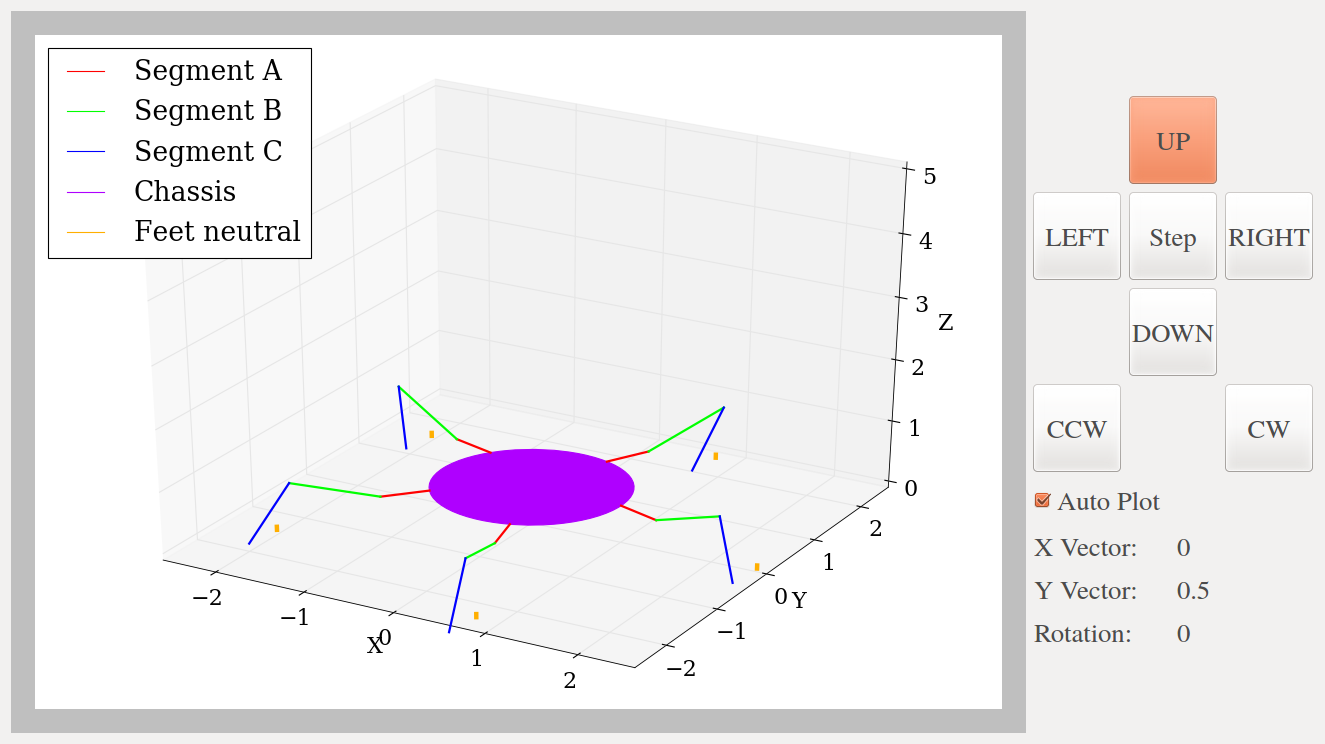
\includegraphics[scale = 0.33]{pics/Sim2.png}
\caption{Simulation window showing the robot moving in a positive $Y$-direction.}
\label{fig:Sim2}
\end{figure}

The robot should also be able to translate in the $X$-direction without making a rotation first. This is illustrated in Figure \ref{fig:Sim3}.

\begin{figure}[H]
\centering
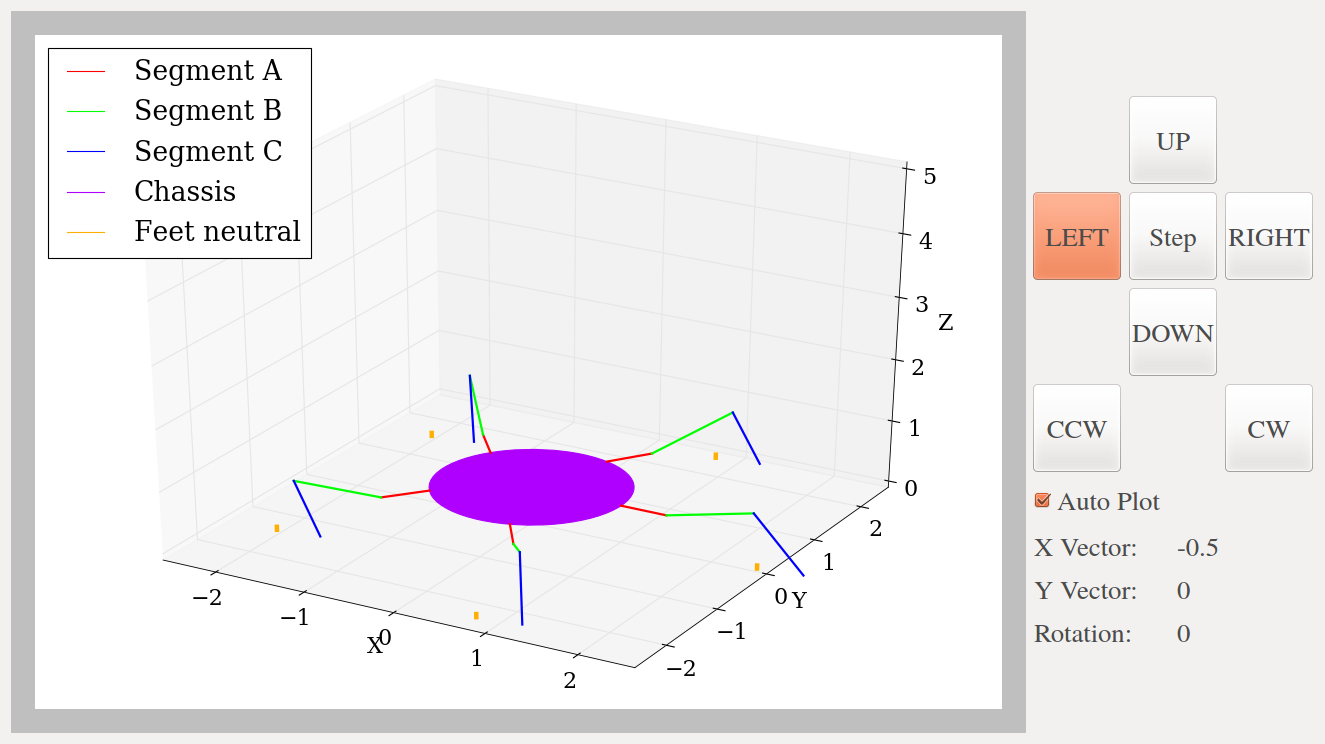
\includegraphics[scale = 0.33]{pics/Sim3.png}
\caption{Simulation window showing the robot moving in a negative $X$-direction.}
\label{fig:Sim3}
\end{figure}

If the robot can instantaneously move in both the $X$ and $Y$-directions, it should be able to move in a combination of the two without a problem. This ability is illustrated in Figure \ref{fig:Sim4}.

\begin{figure}[H]
\centering
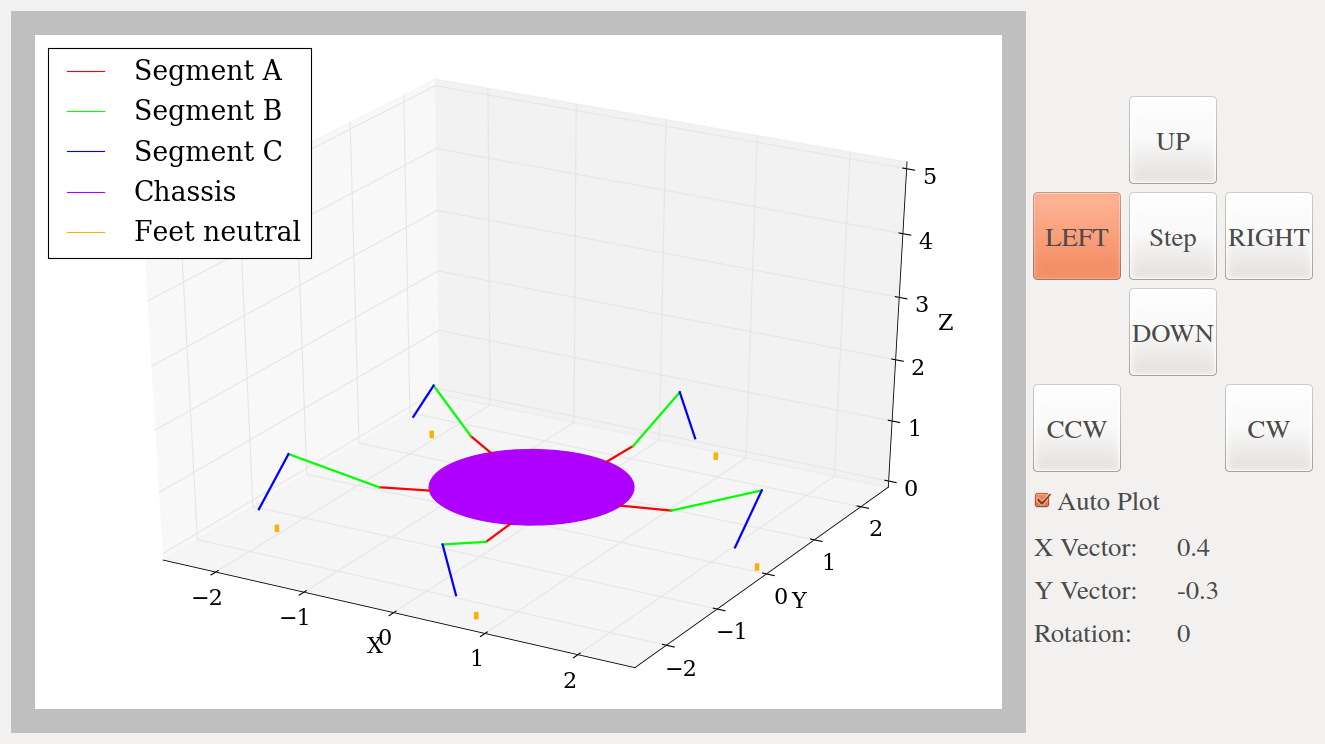
\includegraphics[scale = 0.33]{pics/Sim4.png}
\caption{Simulation window showing the robot moving in a direction with a positive $X$ and negative $Y$-component.}
\label{fig:Sim4}
\end{figure}

The translation appears to be working exactly as intended and designed for. The simulation is tested with a clockwise direction rotation in Figure \ref{fig:Sim5}.

\begin{figure}[H]
\centering
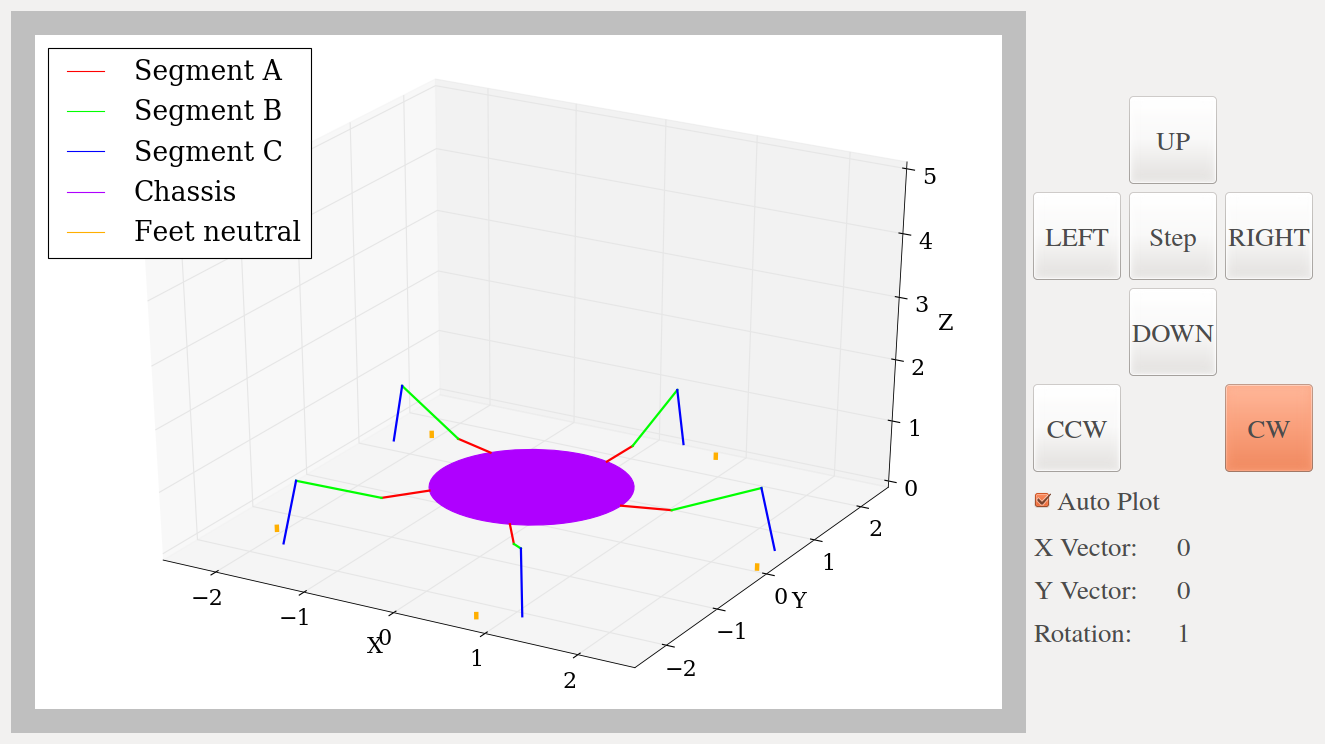
\includegraphics[scale = 0.33]{pics/Sim5.png}
\caption{Simulation window showing the robot rotating in a clockwise direction.}
\label{fig:Sim5}
\end{figure}

Once the robot reaches the boundary illustrated in Figure \ref{fig:Body_layout_3} for any of its legs, it is necessary to lift the leg up, move it to a more suitable location and put it down in order to continue in the direction it is heading in. This ability is illustrated in Figure \ref{fig:Sim6}.

\begin{figure}[H]
\centering
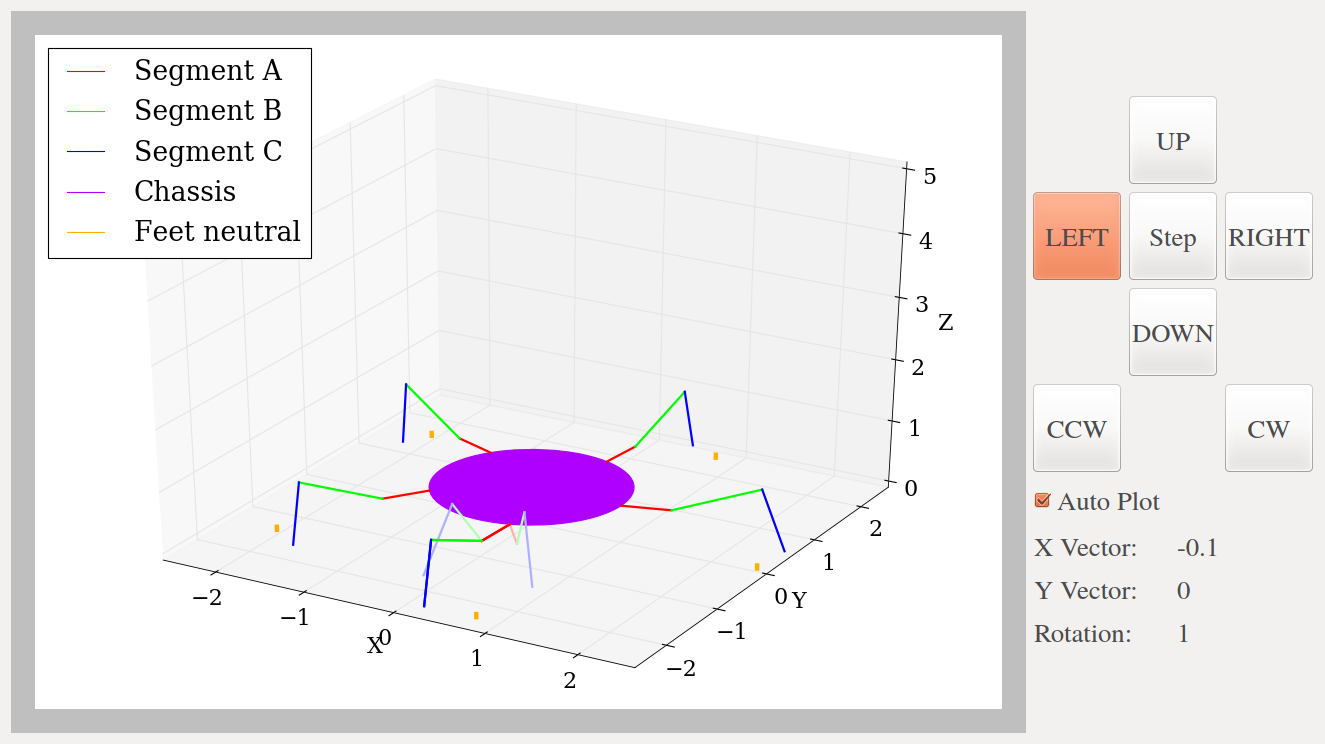
\includegraphics[scale = 0.33]{pics/Sim6.png}
\caption{Simulation window showing the robot picking up a foot and placing it again.}
\label{fig:Sim6}
\end{figure}

In Figure \ref{fig:Sim6}, the closest leg appears three times, twice in dimmed (ghost) colours and then finally in the normal colours. What this attempts to illustrate is the resetting motion of the leg. Figure \ref{fig:Sim5} shows the robot just before the resetting action. The right of the two "ghost" legs is right above the original location of the leg. This shows the position of the leg after it was lifted up. The left of the two "ghost" legs is the leg, still lifted, after being moved to a position directly over the new location. The leg plotted in full colour shows the final position of the leg. It is now able to start rotating further in the clockwise direction. Th robot will pickup and replace one leg at a time for all the legs that requires resetting and then continue.


\subsubsection{Optimisation}

\subsubsection{Hardware design}

\subsubsection{Hardware implementation}

\subsubsection{Software design}

\subsubsection{Software implementation}

\subsubsection{Design summary}


\secun{Results}

\subsubsection{Summary of results achieved}

\begin{tabular}{|p{5cm}|p{5cm}|p{5cm}|}
\hline
\textbf{Description of requirement or specification
(intended outcome)} & \textbf{Actual outcome}& \textbf{Location in report}\\
\hline
\multicolumn{3}{|l|}{}\\
\multicolumn{3}{|l|}{\textbf{Mission requirements of the product}}\\
\hline
1&2&3\\
\hline
\multicolumn{3}{|l|}{}\\
\multicolumn{3}{|l|}{\textbf{Field conditions}}\\
\hline
1&2&3\\
\hline
\multicolumn{3}{|l|}{}\\
\multicolumn{3}{|l|}{\textbf{Specifications}}\\
\hline
1&2&3\\
\hline
\multicolumn{3}{|l|}{}\\
\multicolumn{3}{|l|}{\textbf{Deliverables}}\\
\hline
1&2&3\\
\hline

\end{tabular}

\subsubsection{Qualification tests}
%Just cite something for bibTex to work
\cite{Hidayat:Autonomous}

%% Use the IEEE Transactions style for the references.
\bibliographystyle{IEEEtran}
\bibliography{Final}
\addcontentsline{toc}{section}{References}

\end{document}

%% End of File.
